
\clearpage
\section{Meeting Management}

The 'Meeting Management' function in CUBE PA enables the following activities:

% Probleme aufgetreten von hier bis (Probleme aufgetreten bis da) 5.5.2016

\begin{itemize}
\item
To compose and send a meeting invitation
\item
To compile and send the meeting minutes
\item
To set up and track actions
\item
To document decisions
\item
To look up and read / edit meeting invitations, meeting minutes, actions and decisions
\end{itemize}

\vspace{2cm}

\begin{wrapfigure}[2]{l}{6.5cm}   % [x] Wie manche Zeile soll sich um die Grafik "brechen"
  \vspace{-35pt}      % Grundwert war 20; mit 30 schön oben beim Text ausgerichtet
  \begin{center}
    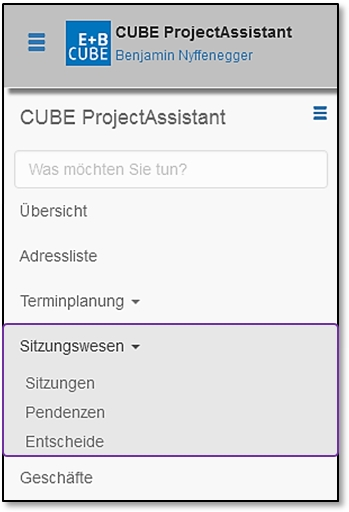
\includegraphics[width=1\linewidth]{../chapters/05_Sitzungswesen/pictures/5-1_Menu_Sitzungswesen.jpg}
  \end{center}
  \vspace{-20pt}
  \caption{Using the meeting management function}
  \vspace{-10pt}
\end{wrapfigure}

In the left-hand menu, select the 'Meeting Management' menu item and then the 'Meetings' sub-item.

\vspace{5cm}

\pagebreak
\textbf{The meeting overview briefly explained:}

\begin{figure}[H]
\center{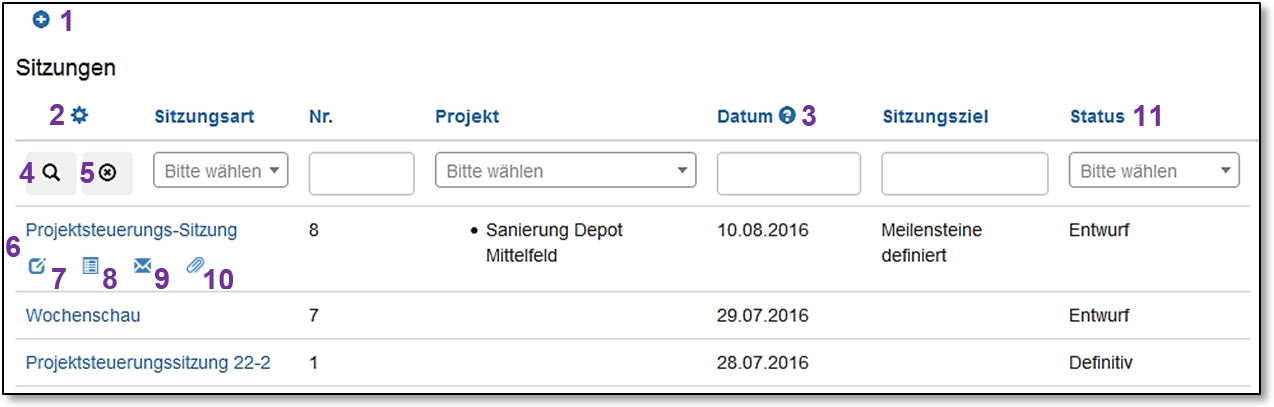
\includegraphics[width=1\linewidth]{../chapters/05_Sitzungswesen/pictures/5_SitzungenUebersicht.jpg}}
\caption{The meeting overview}
% \label{fig:speciation}
\end{figure}

The meeting overview gives a summary of the ongoing or past meetings. Using the plus symbol 
\includegraphics[height=12pt]{/Icons/Plussymbol.jpg} \col{(1)} you can add a new meeting. If too many columns are displayed, you can hide them using the configuration symbol 
\includegraphics[height=12pt]{/Icons/SpaltenEinst.jpg} \col{(2)}. The question mark 
\includegraphics[height=12pt]{/Icons/Fragezeichen.jpg} \col{(3)} gives information about the date formatting and the search options: 

\begin{figure}[H]
\center{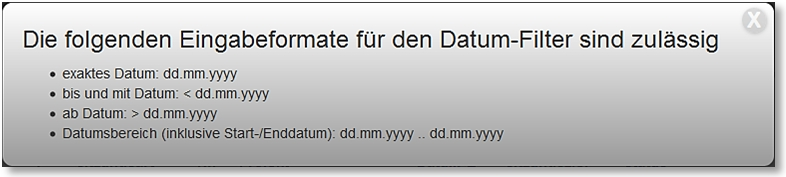
\includegraphics[width=0.7\linewidth]{../chapters/05_Sitzungswesen/pictures/5_Datumformat.jpg}}
% \caption{Das Menü in CUBE PA}
% \label{fig:speciation}
\end{figure}

You can search through the meetings with the filter. Enter keywords or choose a desired entry from one of the drop-down menus (e.g. Project). Then click on the magnifying glass (search) symbol 
\includegraphics[height=12pt]{/Icons/Lupe_s.jpg} \col{(4)}. All found entries are shown. Click on the cross (reset search) 
\includegraphics[height=12pt]{/Icons/FilterLoeschen.jpg} \col{(5)} to delete all filter settings. \\
Click on the column heading to sort the list (by ascending or descending order).

When you click on a meeting title (blue), further options are opened under it \col{(6)}: You can edit a meeting invitation 
\includegraphics[height=12pt]{/Icons/bearbeiten.jpg} \col{(7)}, edit the meeting minutes 
\includegraphics[height=12pt]{/Icons/Listensymbol.jpg} \col{(8)}, open or save the meeting invitation as a PDF file 
\includegraphics[height=12pt]{/Icons/Briefsymbol.jpg} \col{(9)} or if you have attached a document to the meeting invitation, you can click on the paper-clip symbol 
\includegraphics[height=12pt]{/Icons/Bueroklammer.jpg} \col{(10)} to download the document. \\
The status column \col{(11)} shows if meeting minutes have been archived and are thus 'Final'. If a meeting has this status, the above described options are no longer available. Using the sheet symbol 
\includegraphics[height=12pt]{/Icons/Blattsymbol.jpg}, finalized meeting minutes can be opened or saved as a PDF file.

\subsection{Invitation to a meeting}
\label{bkm:Ref434828480}

Click on the plus (add) symbol 
\includegraphics[height=12pt]{/Icons/Plussymbol.jpg} \col{(1)} at the top left.

\vspace{\baselineskip}

\begin{figure}[H]
\center{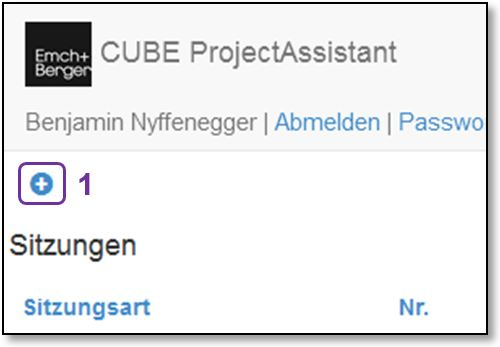
\includegraphics[width=0.4\linewidth]{51_Neue_Sitzung.jpg}}
\caption{Adding a new meeting}
% \label{fig:speciation}
\end{figure}

% \vspace{\baselineskip}

The form for entering a new meeting appears:

\begin{figure}[H]
\center{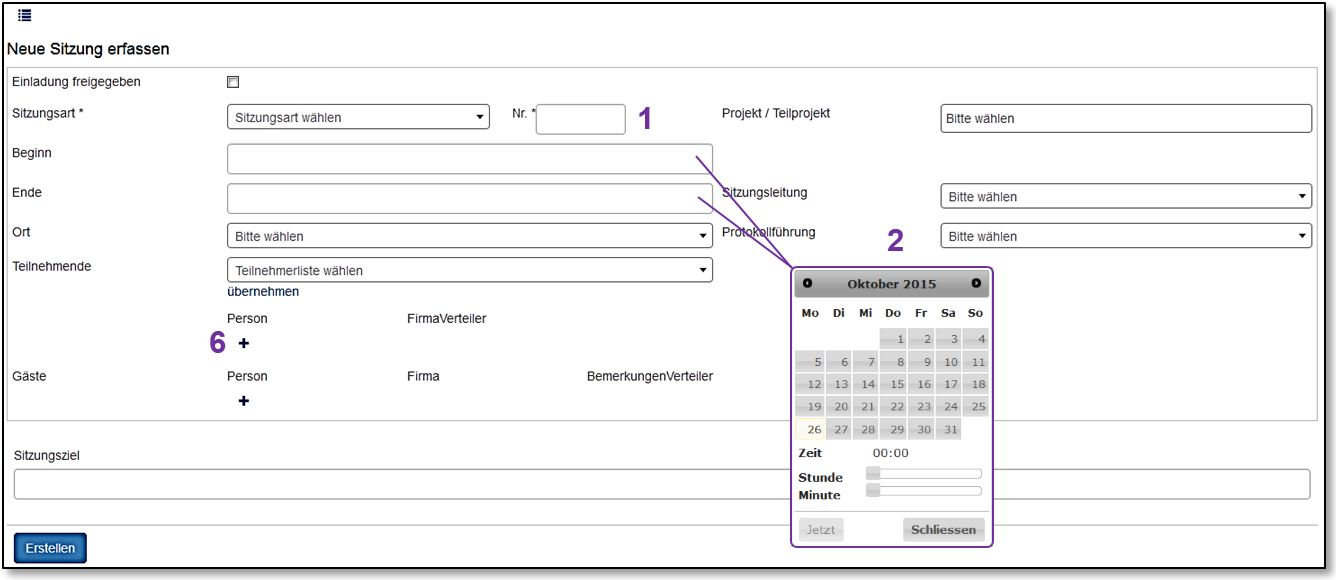
\includegraphics[width=1\linewidth]{51_Neue_Sitzung_erfassen.jpg}}
\caption{Recording a new meeting}
% \label{fig:speciation}
\end{figure}

\begin{figure}[H]
\center{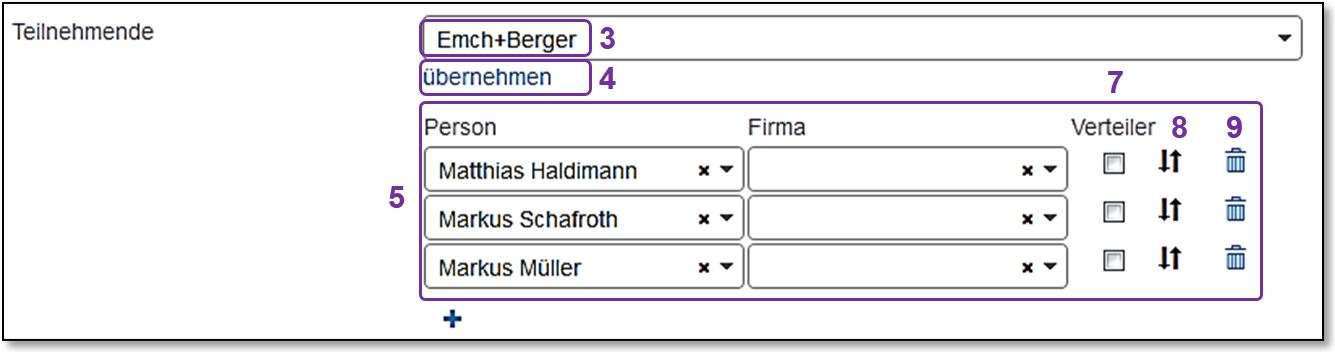
\includegraphics[width=1\linewidth]{51_Neue_Sitzung_Teilnehmende.jpg}}
\caption{Selecting meeting participants}
% \label{fig:speciation}
\end{figure}

Fill in the form; mandatory fields are marked with an asterisk (*). The following points are important:

\begin{itemize}
\item 
When you select a meeting type, CUBE PA automatically sets the corresponding number \col{(1)}.
\item 
When you click in the fields 'Start' and 'End', a calendar appears, in which the date and time can be selected \col{(2)}.
\item 
In the field 'Meeting Participants' you can can select a ready-made participant list \col{(3)} that contains all usual participants. Then click immediately on 'apply' \col{(4)} and the list of all participants appears below \col{(5)}.
\item 
If an additional participant not on the list is to take part in the meeting, or if the participants are to be put together on an ad hoc basis, click on the plus (add) sign \col{(6)} underneath the 'Meeting Participants' field and select the appropriate information in the 'Person' and 'Company' fields. 
\item
Check the check-box \col{(7)} under 'Distribution' if the participant should appear in the distribution list.
\item 
If the order of the participants needs to be changed, drag the symbol with two opposing vertical arrows 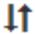
\includegraphics[height=12pt]{/Icons/VertPfeile.jpg} \col{(8)} next to the participant and drop it in the correct position.
\item 
By clicking on the garbage bin (remove) symbol 
\includegraphics[height=12pt]{/Icons/Muelltonne.jpg} \col{(9)} you can remove a participant. Confirm the warning message 'Remove?' with 'OK'.
\item 
If the meeting has a guest, e.g. for a special agenda item, you can add the guest in the section 'Guests' by clicking on the plus (add) sign and choosing the appropriate information in the 'Person' and 'Company' fields. The symbols in this section have the same functions as in the 'Meeting Participants' section.
\item 
If a person who does not appear in the above-mentioned selections is to take part in the meeting, you must enter them in 'User Management' (see chapter \ref{bkm:Ref434828324}). If a required person is missing from a predefined list of people, you can add that person via the menu item 'Configuration', then 'Meeting Participants', provided that the person has already been registered in the user management.
\end{itemize}

Once you have entered all the data, click on the 'Create' button 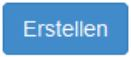
\includegraphics[height=12pt]{/Icons/B_Erstellen.jpg} at the bottom left.

\begin{figure}[H]
\center{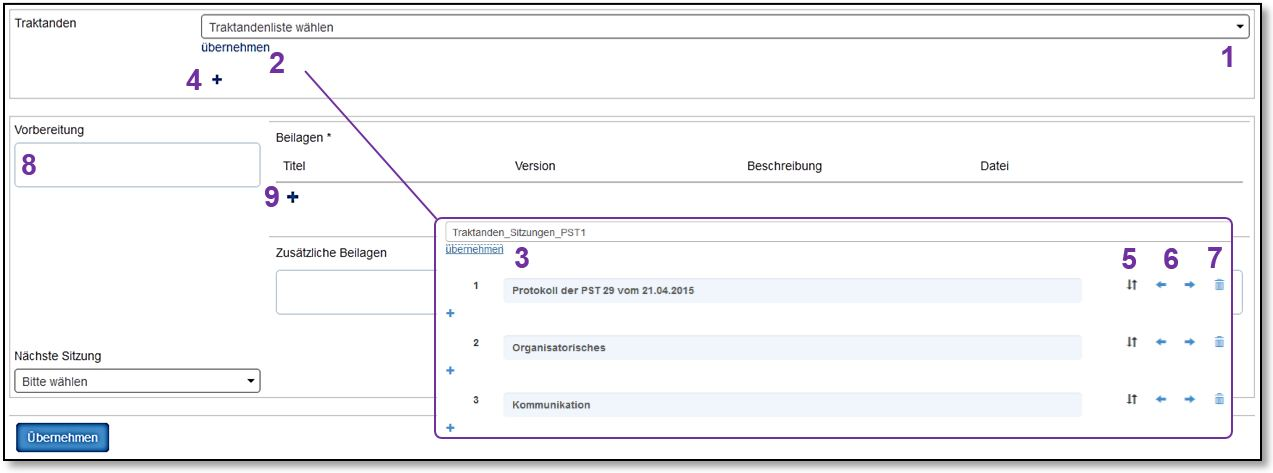
\includegraphics[width=1\linewidth]{51_Traktanden.jpg}}
\caption{Inserting agenda items}
% \label{fig:speciation}
\end{figure}

The following points are important:

\begin{itemize}
\item 
In the 'Agenda Items' field you can choose a ready-made agenda items list \col{(1)}, and then click on 'apply' \col{(2)}. The complete list of agenda items is then displayed \col{(3)}. As with the meeting participants, you can click on the plus (add) sign \col{(4)} to add additional agenda items as free text, and use the symbol with opposing vertical arrows \col{(5)} to change the order of items. Clicking on the horizontal arrow \col{(6)} enables you to set an item higher or lower in the numbering hierarchy. If a previously defined agenda item needs to be removed, click on the garbage bin symbol 
\includegraphics[height=12pt]{/Icons/Muelltonne.jpg} \col{(7)} and confirm the security warning.
\item 
In the 'Preparation' field, you can enter preparations with free text \col{(8)}. Preparations are to be understood as activities to be carried out in preparation for a meeting, e.g. preparing a presentation.
\end{itemize}

\begin{figure}[H]
\center{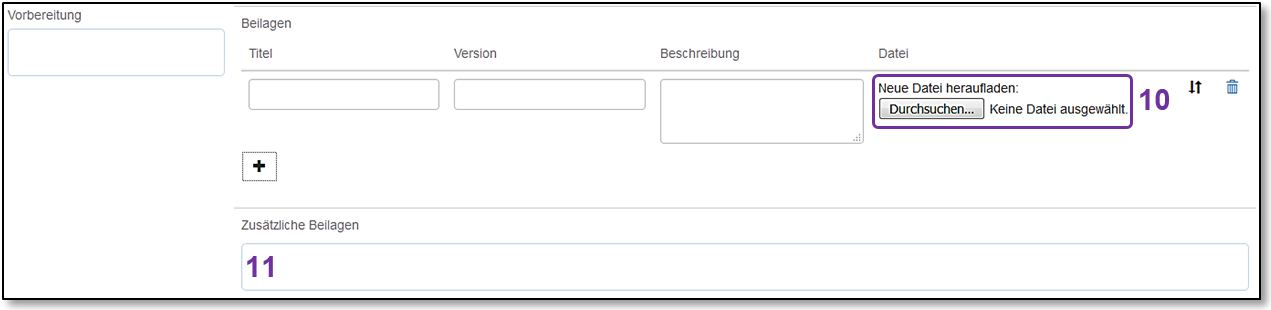
\includegraphics[width=1\linewidth]{51_Vorbereitung.jpg}}
\caption{Uploading attachments}
% \label{fig:speciation}
\end{figure}

\begin{itemize}
\item 
If you want to attach documents to the meeting invitation, click on the plus (add) sign under 'Attachments' \col{(9)}. You can then enter the title, version and description of the attachment. Click on 'Browse' under 'Upload new file' \col{(10)}. Choose the desired attachment and click 'Open'. The attachment will appear in the personal overview of every participant who uses CUBE PA. Use the symbol with opposing vertical arrows to change the order of the attached files. Click on the garbage bin symbol 
\includegraphics[height=12pt]{/Icons/Muelltonne.jpg} to remove an attachment. After the upload, the file and the file name become visible:
\end{itemize}

\begin{figure}[H]
\center{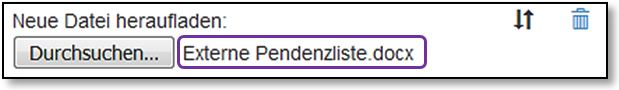
\includegraphics[width=0.5\linewidth]{51_NeueDateiHochladen.jpg}}
\caption{The uploaded file is visible}
% \label{fig:speciation}
\end{figure}

\textbf{Tip:} Instead of clicking on 'Browse' and selecting the document, you can drag and drop the file over the 'Browse' field. The file will be uploaded and linked to the meeting invitation.

\vspace{\baselineskip}

\begin{itemize}
\item 
Additional Attachments \col{(11)}: In this section, additional attachments which haven't been uploaded to CUBE PA and are therefore not available (e.g. plans in paper format) can be mentioned.
\item 
In the 'Follow up Meeting' field you can simply select the next meeting and it will appear in the invitation with its place and time. This presupposes however that the next meeting is already recorded in an invitation.
\end{itemize}

Having filled out all the information, click on the 'Update' button 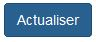
\includegraphics[height=12pt]{/Icons/B_Uebernehmen.jpg}. \newline
Scroll back to the top and click on the letter symbol 
\includegraphics[height=12pt]{/Icons/Briefsymbol.jpg} at the top left. The finished invitation appears in PDF format. You can now save the invitation on your PC and send it by e-mail or by post to the meeting participants.

\vspace{\baselineskip}

Releasing the meeting invitation to the personal overview page:

\begin{itemize}
\item
To share the meeting invitation with its list of actions and possible attachments to the personal overview pages of the invitees, the corresponding check-box in the input form above the meeting type field must be checked:
\end{itemize}

\begin{figure}[H]
\center{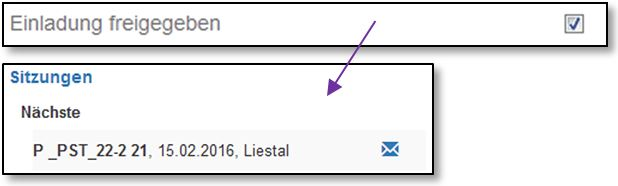
\includegraphics[width=0.5\linewidth]{51_EinladungFreigeben.jpg}}
\caption{Release invitation}
% \label{fig:speciation}
\end{figure}

\begin{small}
The 'Invitation released' check-box was checked when creating the meeting invitation. The letter symbol is visible in the personal overview.
\end{small}

\begin{itemize}
\item
If the check-box was not checked, the time and place are shown for the users, but the list of actions and the attachments are not available to download.
\end{itemize}

\begin{figure}[H]
\center{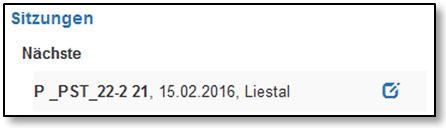
\includegraphics[width=0.5\linewidth]{51_SitzungenBearbeiten.jpg}}
\caption{Editing a meeting invitation}
% \label{fig:speciation}
\end{figure}

\begin{small}
The 'Invitation released' check-box was not checked when creating the meeting invitation. The invitation can be edited by clicking on the editing symbol in the personal overview.
\end{small}

% Probleme aufgetreten bis da (Code könnte genommen werden von: 20160505_1724_LaTeX Document (neu)V2
% scheint, aber gut zu sein 5.5.2016, bny
% alle \liststyle etc... gelöscht Fehler von 143 auf 89 reduziert.

\subsection{Recording the meeting minutes}

There are two options for recording the meeting minutes:

\begin{enumerate}
\item
You can record the meeting minutes directly in CUBE PA. This requires a working Internet connection during the meeting and is especially recommended when all meeting participants use CUBE PA and use it for their comments on the meeting minutes. 
It is of course also possible to make simple notes during the meeting and then enter the meeting minutes later in CUBE PA.
\item
You can record the meeting minutes in a document outside CUBE PA and upload the approved meeting minutes to CUBE PA. 
This procedure is appropriate in cases when the discussion does not follow the agenda items given out with the meeting invitation or is simply unstructured, or when many of the meeting participants do not use CUBE PA.
\end{enumerate}

For some projects, it is important to have a clear record of who has made changes to the meeting minutes. CUBE PA disposes of an editing mode that records who has made which changes, but its use is optional, like the editing mode in Microsoft Word. 
In the end it is up to the users to keep track of the changes.

\subsubsection{Recording the meeting minutes in CUBE PA}

Once you are in the meeting room, check if the Internet connection is available and if you have access to CUBE PA. The connection symbol at the bottom right must not be red.

\vspace{\baselineskip}

From the menu, select the 'Meeting Management' menu item and the subcategory 'Meetings'. The list of meetings recorded in CUBE PA appears, that is, meetings for which an invitation has been created in CUBE PA at least. 

\begin{figure}[H]
\center{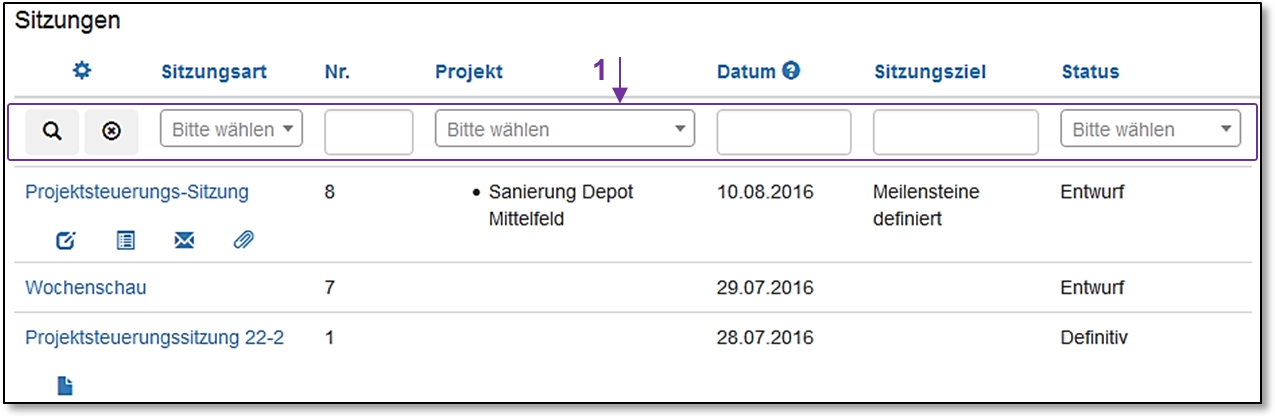
\includegraphics[width=1\linewidth]{../chapters/05_Sitzungswesen/pictures/5-2-1_SitzungenListe.jpg}}
\caption{Overview of recorded meetings}
% \label{fig:speciation}
\end{figure}

\textbf{Filter function}\col{(1)}

Use the filter function to find the desired meeting. Fill in the fields marked above with what you know or what you are looking for. Then click on the magnifying glass (search) symbol 
\includegraphics[height=12pt]{/Icons/Lupe_kl.jpg} or hit 'Enter'.

\vspace{\baselineskip}

All entries which match the search terms are displayed. In the meeting goal field you can enter any keywords that appear in the meeting goal (you do not need to use a placeholder * before a word).

\vspace{\baselineskip}

\textbf{Legend for editing meeting entries}

\vspace{\baselineskip}

\begin{tabular}{|c|p{14cm}|} %{cl}
\hline
\raisebox{-1\totalheight}{
\includegraphics[height=12pt]{/Icons/Blattsymbol.jpg}} & The meeting minutes have been 'archived' and can no longer be edited, but only viewed \\
\hline
\raisebox{-.25\totalheight}{
\includegraphics[height=12pt]{/Icons/Bearbeiten.jpg}} & Editing the meeting invitation, see chapter \ref{bkm:Ref434828480} \\
\hline
\raisebox{-.25\totalheight}{
\includegraphics[height=12pt]{/Icons/Listensymbol.jpg}} & Editing the meeting minutes\\
\hline
\raisebox{-.25\totalheight}{
\includegraphics[height=12pt]{/Icons/Briefsymbol.jpg}} & Opening the meeting invitation as a PDF file (for sending by e-mail or post) \\
\hline
\raisebox{-.25\totalheight}{
\includegraphics[height=12pt]{/Icons/Bueroklammer.jpg}} & There are attachments with this meeting invitation \\
\hline
\end{tabular}

\vspace{\baselineskip}

Locate the meeting in question in the list and click on the list symbol 
\includegraphics[height=12pt]{/Icons/Listensymbol.jpg} on the right. The input form for entering the meeting minutes appears.

\begin{figure}[H]
\center{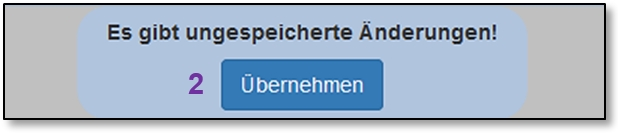
\includegraphics[width=0.4\linewidth]{../chapters/05_Sitzungswesen/pictures/5-2-1_Uebernehmen_top.jpg}}
% \caption{Das Menü in CUBE PA}
% \label{fig:speciation}
\end{figure}

\begin{figure}[H]
\vspace{-20pt}  
\center{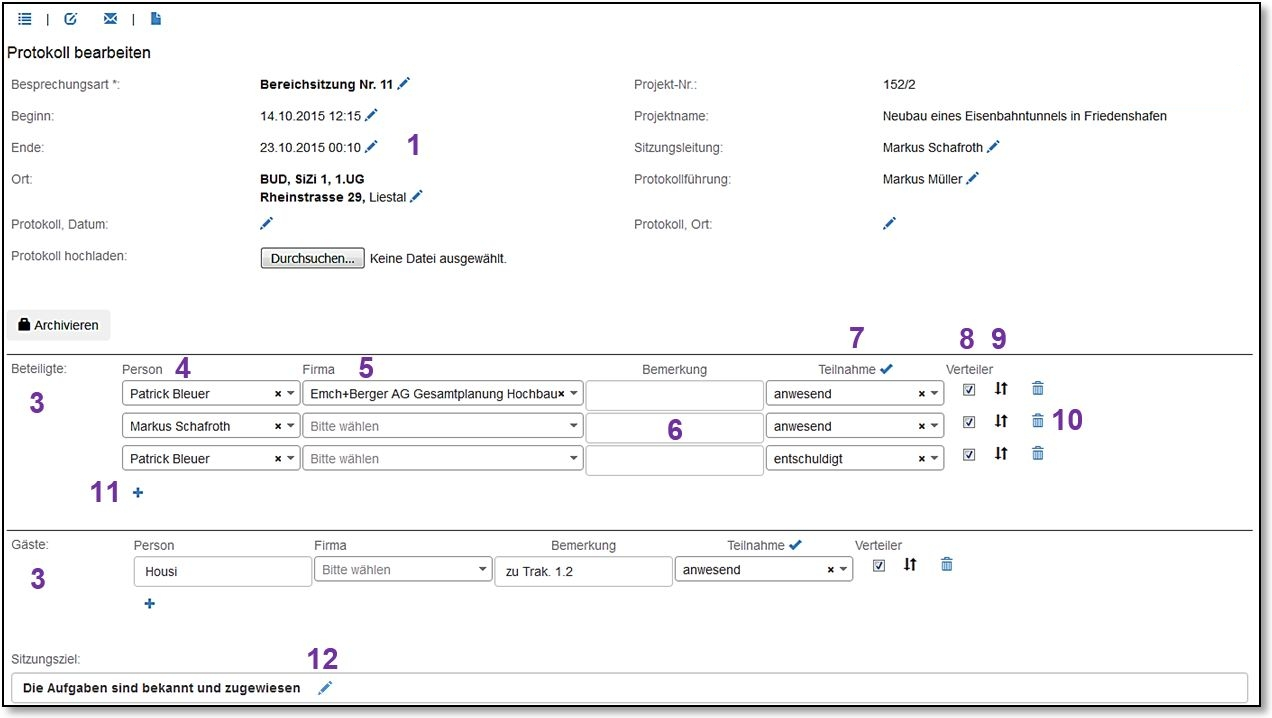
\includegraphics[width=1\linewidth]{../chapters/05_Sitzungswesen/pictures/5-2-1_ProtokollBearbeiten.jpg}}
\caption{Editing meeting minutes}
% \label{fig:speciation}
\end{figure}

\begin{itemize}
\item
Meeting type, start, end, location, project number, project name, meeting moderator, and meeting secretary in the top part of the form are automatically filled out with the information from the invitation. If you want to edit this information, click on the pen symbol 
\includegraphics[height=12pt]{/Icons/Stift.jpg} \col{(1)} usually found next to the field in question and change the information. The location and date each have a field: with calendar selection for the date and with list selection for the location. Click on the 'Update' button \col{(2)} (bottom left of the page, or top middle) to save the changes.
\item
For the 'Meeting Participants' and 'Guests' sections \col{(3)}, making changes functions in the same way as when preparing the meeting invitation. Click on on the fields 'Person' \col{(4)} or 'Company' \col{(5)}, and you get a selection list from which you can select another person or another company. In the 'Remark' field \col{(6)} you can enter comments as free text, like for example 'only absent until 9 o’clock'. In the 'Participation' field \col{(7)} you can choose between 'attended' and 'did not attend'. Check the 'Distribution' check-box \col{(8)} to add someone to the distribution list. Use the symbol with opposing vertical arrows 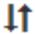
\includegraphics[height=12pt]{/Icons/VertPfeile.jpg} \col{(9)} to change the order of the participants in the list.
\item
Click on the garbage bin symbol 
\includegraphics[height=12pt]{/Icons/Muelltonne.jpg} \col{(10)} to remove a participant. Click on the plus symbol 
\includegraphics[height=12pt]{/Icons/Pluszeichen.jpg} \col{(11)} to add a participant.
\item
Editing, adding and removing guests works the same way as with participants.
\item
You can edit the goal of the meeting by clicking on the pen symbol 
\includegraphics[height=12pt]{/Icons/Stift.jpg} \col{(12)}.
\item
To save the changes click on the 'Update' button \col{(2)}.
\end{itemize}

The list of agenda items from the invitation appears under the goal of the meeting.

\begin{figure}[H]
\center{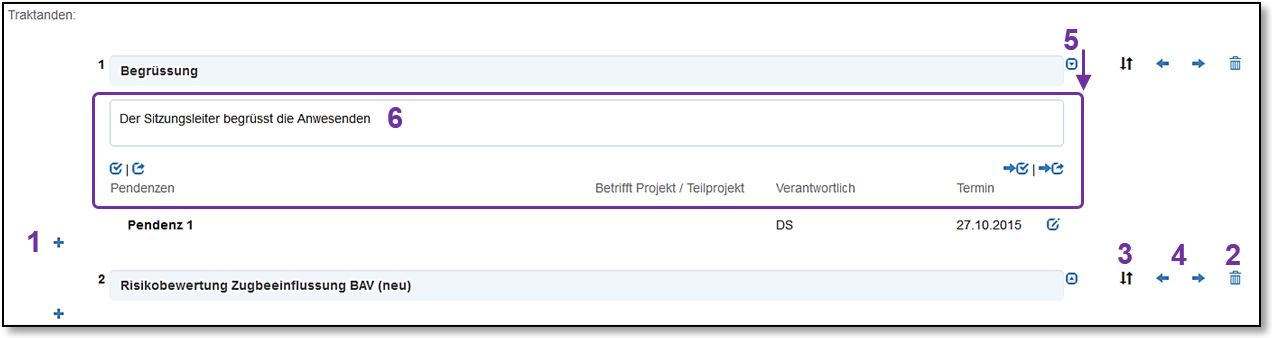
\includegraphics[width=1\linewidth]{521_Traktanden.jpg}}
\caption{List of agenda items}
% \label{fig:speciation}
\end{figure}

In this section you can enter the meeting minutes text as well as enter decisions and actions.

\begin{itemize}
\item
You can edit the list of agenda items the same way as when preparing the invitation: By clicking on the plus sign 
\includegraphics[height=12pt]{/Icons/Pluszeichen.jpg} \col{(1)} an additional agenda item is created, and by clicking on the garbage bin symbol 
\includegraphics[height=12pt]{/Icons/Muelltonne.jpg} \col{(2)} an agenda item is removed. If you want to change the order of the agenda items, use the vertical opposing arrows symbol 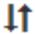
\includegraphics[height=12pt]{/Icons/VertPfeile.jpg} \col{(3)} next to an item.
\item
Clicking on the horizontal arrows 
\includegraphics[height=12pt]{/Icons/Pfeil-links-rechts.jpg} \col{(4)} to change the structure:

	\begin{itemize}
		\item
		The standard classification is 1, 2, 3 etc. \col{(a)}
		\item
		Click once on the right-pointing arrow 
\includegraphics[height=12pt]{/Icons/Pfeil-rechts.jpg} \col{(b)}, and the selected row is moved under point 1 and numbered 1.1 \col{(c)}.
		\item
		If you don't want a numbered structure but instead only want one paragraph under a single agenda item, click again on the right-pointing arrow \includegraphics[height=12pt]{/Icons/Pfeil-rechts.jpg} \col{(d)}: The row is no longer numbered and a regular paragraph is created under the above numbering \col{(e)}.
		\item
		Clicking on the left-pointing arrow \includegraphics[height=12pt]{/Icons/Pfeil-links.jpg} \col{(f)} allows you to undo the changes.
	\end{itemize}
\end{itemize}

\begin{figure}[H]
\center{\includegraphics[width=1\linewidth]{521_Protokoll_ordnen.jpg}}
\caption{Structure of the meeting minutes}
% \label{fig:speciation}
\end{figure}

To enter the meeting minutes text of an agenda item, click on the expansion sign \includegraphics[height=12pt]{/Icons/Aufklappen.jpg} \col{(5)} (a small triangle in a square) next to the label of the agenda item. A text box in which you can enter free text for this agenda item \col{(6)} appears.

\vspace{\baselineskip}

The four symbols below the text box open the following possibilities:

\begin{figure}[H]
\center{\includegraphics[width=1\linewidth]{521_EntscheidSymbole.jpg}}
\caption{Further options for the decisions}
% \label{fig:speciation}
\end{figure}

\begin{itemize}
\item
Do you want to enter a decision that should automatically be included in the decision list? Click on the symbol on the left \includegraphics[height=12pt]{/Icons/Gutzeichen_Rahmen.jpg} \col{(a)} and a window appears in which you can enter the decision. The fields 'Title' \col{(1)} and 'Description' \col{(2)} are free text fields. The 'Project / Subproject' field \col{(3)} is a drop-down list for selecting the corresponding project or subproject. Click on the 'Create' button \col{(4)} to save the decision or on the cross \col{(5)} to discard the entry.

\begin{figure}[H]
\center{\includegraphics[width=0.75\linewidth]{521_EntscheidHinzufuegen.jpg}}
\caption{Adding a decision}
% \label{fig:speciation}
\end{figure}

\end{itemize}

\begin{itemize}
\item
Do you want to enter an action that should automatically be included in the list of actions? Click on the second symbol from the left \includegraphics[height=12pt]{/Icons/Pfeil_aus_Box.jpg} \col{(b)} and a window appears in which you can enter the action. The fields 'Title' \col{(1)} and 'Description' \col{(2)} are free text fields. The 'Due Date' field \col{(3)} is a calender from which the date can be selected. In the remaining fields \col{(4)} data can be selected from a list. Click on the 'Create' button \col{(5)} to save the action or on the cross \col{(6)} to discard the entry.

\begin{figure}[H]
\center{\includegraphics[width=0.75\linewidth]{521_PendenzHinzufuegen.jpg}}
\caption{Adding an action}
% \label{fig:speciation}
\end{figure}

\end{itemize}

\begin{figure}[H]
\center{\includegraphics[width=1\linewidth]{521_EntscheidSymbole2.jpg}}
\caption{Converting agenda items into decisions or actions}
% \label{fig:speciation}
\end{figure}

\begin{itemize}
\item
Saved decisions and actions appear on the screen directly below the relevant agenda item.
\item
You realized that the text you entered as an agenda items is actually a decision? Click on the second symbol from the right \includegraphics[height=12pt]{/Icons/Pfeil_Gutzeichen.jpg} \col{(c)} and the text appears in a window in which you can complete the information as a decision and save it. \textbf{Warning}: The text will be moved to the decision window, not copied!
\item
You realized that the text you entered as an agenda item is actually an action? Click on the symbol on the right \includegraphics[height=12pt]{/Icons/Pfeil_Pfeil_aus_Box.jpg} \col{(d)} and the text appears in a window in which you can complete the information as an action and save it. \textbf{Warning}: The text will be moved to the action window, and not copied!
\end{itemize}

% \vspace{\baselineskip}

\textbf{Tip}: It is not necessary to enter the meeting minutes in a perfectly structured manner as described above during the meeting. Copy-paste functions just like in Microsoft Word: Select the text you want to copy and use either a right-click (context menu) or the shortcuts 'Ctrl+C' (copy), 'Ctrl+X' (cut) and 'Ctrl+V' (paste). You can for example write all the text in the first agenda item then divide it over the different agenda items after the meeting. Entering decisions and actions is also possible later in the course of recording the meeting minutes.

\vspace{\baselineskip}

\textbf{Formatting meeting minutes:}

% \vspace{\baselineskip}

As soon as you click in a meeting minutes text field, a ribbon with formatting buttons appears \col{(1)}. These function like the similar buttons in Microsoft Word:

\begin{figure}[H]
\center{\includegraphics[width=1\linewidth]{521_TextFormatieren.jpg}}
\caption{Formatting text}
% \label{fig:speciation}
\end{figure}

\begin{compactitem}
\item Bold: displays selected text in bold
\item Italic: displays selected text in italics
\item Underlined: underlines selected text
\item Background color: colors the background the the selected text
\item Superscript: superscripts selected text
\item Remove formatting: removes all formatting from the selected text
\item Insert from MS-Word: pastes text which you have selected and copied 
in Microsoft Word directly into the text field
\item Undo: undoes the last change
\item Redo: restores an undone change
\item Numbered list: converts selected lines 
into a numbered list
\item List: converts selected lines into 
a list with bullet points
\item Reduce indent: moves the selected text to the left
\item Increase indent: moves the selected text to the right
\item Insert table: inserts a table at the current cursor position. 
A window appears in which you can set the table parameters. 
Experiment with the possibilities.
\end{compactitem}

\vspace{\baselineskip}

\begin{sloppypar}
To the right of these formatting buttons are buttons for the revision mode. This function is explained in chapter \ref{bkm:Ref434478117}.
\end{sloppypar}

\subsubsection{Uploading the meeting minutes as a document}

Prepare the meeting minutes as a document, e.g. with Microsoft Word, and have it checked the conventional way by the rest of the participants. As soon as you have a final version of the meeting minutes, generate a PDF file of the minutes and upload it into CUBE PA:

\vspace{\baselineskip}

\begin{wrapfigure}[7]{l}{6.5cm}   % [x] Wie manche Zeile soll sich um die Grafik "brechen"
  \vspace{-35pt}      % Grundwert war 20; mit 30 schön oben beim Text ausgerichtet
  \begin{center}
    \includegraphics[width=1\linewidth]{../chapters/05_Sitzungswesen/pictures/5-1_Menu_Sitzungswesen.jpg}
  \end{center}
  \vspace{-20pt}
  \caption{The meeting management}
  \vspace{-10pt}
\end{wrapfigure}

Select the 'Meeting Management' menu item and then the 'Meetings' sub-item in the menu on the left. A list of meetings recorded in CUBE PA appears, that is, meeting for which for which an invitation has been created in CUBE PA at least. \newline

\vspace{6.5cm} 

Search for the relevant meeting in the list and click on the 'Edit minutes of meeting' symbol \includegraphics[height=12pt]{/Icons/Listensymbol.jpg} \col{(1)} on the left:

\begin{figure}[H]
\center{\includegraphics[width=1\linewidth]{../chapters/05_Sitzungswesen/pictures/5-2-2_Sitzungsuebersicht.jpg}}
\caption{Meetings overview}
% \label{fig:speciation}
\end{figure}

\vspace{\baselineskip}

The form for entering the meeting minutes appears:

\begin{figure}[H]
\center{\includegraphics[width=1\linewidth]{../chapters/05_Sitzungswesen/pictures/5-2-2_ProtokollErfassen.jpg}}
\caption{Entering meeting minutes}
% \label{fig:speciation}
\end{figure}

\textbf{Tip:} Instead of clicking on 'Browse' under 'Upload Minutes' and selecting the minutes, you can drag and drop the file over the 'Browse' field. The minutes will be uploaded and linked to the meeting invitation.

\vspace{\baselineskip}

\begin{itemize}
\item
Meeting type, start, end, location, project number, project name, meeting moderator, and meeting secretary in the top part of the form are automatically filled out with the information from the invitation. If you want to edit this information, click on the pen symbol \includegraphics[height=12pt]{/Icons/Stift.jpg} \col{(1)} usually found next to the field in question and change the information. The location and date \col{(2)} each have a field: with calendar selection for the date and with list selection for the location. Click on the 'Update' button \col{(3)} (bottom left of the page, or top middle) to save the changes. It is not absolutely necessary that all fields be filled out. Fill out the fields that will allow you to uniquely identify the meeting.
\item
Now click on 'Browse' \col{(4)} under 'Upload Minutes' and double-click to select the PDF file of the meeting minutes. Then click on 'Update'. The information 'Minutes are attached as file' appears in red \col{(5)} and the process ends. If you have uploaded the wrong document, you can delete it by clicking the garbage bin symbol. You can upload a new document afterwards.
\end{itemize}

\vspace{\baselineskip}

\textbf{Warning:} Only PDF documents are supported. If for example a word document is uploaded, an error message will appear when trying to open it in a PDF reader.

\vspace{\baselineskip}

By uploading the document, all CUBE PA users can read the meeting minutes anytime and anyplace, as if it were recorded using CUBE PA. When you are sure that everything in the meeting minutes checks out, click on the 'Archive' button \col{(6)} and confirm the query \col{(7)}. CUBE PA sets the status of this meeting as 'Final'. The minutes for this meeting can no longer be edited and no new minutes can be uploaded.

\begin{figure}[H]
\center{\includegraphics[width=0.5\linewidth]{522_Archivieren.jpg}}
\caption{Archiving meeting minutes}
% \label{fig:speciation}
\end{figure}

\subsubsection{Adding attachments to meeting minutes}

The section for uploading attachments is located under the section for entering the meeting minutes text.

\begin{figure}[H]
\center{\includegraphics[width=1\linewidth]{../chapters/05_Sitzungswesen/pictures/5-2-3_ProtokollBeilagen.jpg}}
\caption{Uploading attachments to meeting minutes}
% \label{fig:speciation}
\end{figure}

The procedure is similar to uploading the minutes as a document:

\begin{itemize}
\item
Click on the plus sign \includegraphics[height=12pt]{/Icons/Pluszeichen.jpg} \col{(1)} to add a new attachment.
\item
Fill in the 'Title', 'Version' and 'Description' fields \col{(2)} as needed.
\item
Now click on 'Browse' \col{(3)} under 'Upload new file' and double-click to select a file. If you have uploaded the wrong document, just upload a new one. Then click on 'Update'.
\item
Use the vertical opposing arrows symbol \includegraphics[height=12pt]{/Icons/VertPfeile.jpg} \col{(4)} to change the order of the attachments. Click on the garbage bin symbol \includegraphics[height=12pt]{/Icons/Muelltonne.jpg} \col{(5)} to remove an attachment.
\end{itemize}

\vspace{\baselineskip}

\textbf{Tip:} Instead of clicking on 'Browse' and selecting the document, you can drag and drop the file over the 'Browse' field. The file will be uploaded and linked to the meeting invitation.

\vspace{\baselineskip}

\textbf{Note}: The attachments are not automatically attached to the PDF version of the meeting minutes. The only purpose of uploading the attachments is to make them accessible to the CUBE PA users.

\subsection{Having the meeting minutes checked by participants and finalized}
\label{bkm:Ref434478117}
If you have entered the meeting minutes in CUBE PA, the participants can check and review them. The meeting minutes can then be finalized.

\vspace{\baselineskip}

In order to check and review the meeting minutes, select 'Meeting Management' and then 'Meetings' in the menu on the left. A list of meetings recorded in CUBE PA appears. A similar list also appears in the personal overview. As long as the concerned meeting has the status 'Draft', the meeting minutes can be modified. Now click on the 'Edit minutes of meeting' symbol \includegraphics[height=12pt]{/Icons/Listensymbol.jpg} \col{(1)} on the left.

\begin{figure}[H]
\center{\includegraphics[width=1\linewidth]{../chapters/05_Sitzungswesen/pictures/5-2-2_Sitzungsuebersicht.jpg}}
\caption{Meetings overview}
% \label{fig:speciation}
\end{figure}

\vspace{\baselineskip}

Now you can modify all the fields. If you want to track which user has made which changes, the revision mode should be used. This works as follows:

\vspace{\baselineskip}

When you click in a text field, a ribbon with buttons appears \col{(1)}. These function the same way as similar buttons in Microsoft Word. The right-hand button block controls the revision mode:

\begin{figure}[H]
\center{\includegraphics[width=1\linewidth]{53_Ueberarbeitungsmodus.jpg}}
\caption{Turning on the revision mode}
% \label{fig:speciation}
\end{figure}

\begin{itemize}
\item
Turning the revision mode on / off \col{(2)}: Clicking on this button turns the revision mode on and off again. After activating the revision mode, changes you have made will be marked \col{(3)} and CUBE PA documents who has made these changes and when \col{(4)}.
\end{itemize}

\begin{figure}[H]
\center{\includegraphics[width=1\linewidth]{53_UeberarbeitungsmodusReferenz.jpg}}
\caption{Revision reference}
% \label{fig:speciation}
\end{figure}

The other buttons are important for finalizing the meeting minutes.

\begin{figure}[H]
\center{\includegraphics[width=.75\linewidth]{53_Formatierungen.jpg}}
\caption{Finalizing the meeting minutes}
% \label{fig:speciation}
\end{figure}

\begin{itemize}
\item
Accept all changes \col{(5)}: all changes within the text field are accepted.
\item
Accept change \col{(6)}: accepts the selected change.
\item
Reject all changes \col{(7)}: all changes within the text field are rejected.
\item
Reject change \col{(8)}: the selected change is rejected.
\end{itemize}

\vspace{\baselineskip}

Before finalizing the meeting minutes, you can generate a PDF version to check the minutes and read them calmly. There is a group of four symbols at the top left of the 'Edit Minutes of Meeting' view. Click on the sheet symbol \includegraphics[height=12pt]{/Icons/Blattsymbol.jpg} \col{(1)} on the right to create a PDF version of the minutes.

\begin{figure}[H]
\center{\includegraphics[width=1\linewidth]{53_ProtokollArchivieren.jpg}}
\caption{Archiving meeting minutes}
% \label{fig:speciation}
\end{figure}

When you are sure that everything in the meting minutes checks out, click on the 'Archive' button \col{(2)} and confirm the query \col{(3)}. CUBE PA sets the status of this meeting as 'Final'. The minutes for this meeting can no longer be edited.

\subsection{Creating actions}

You can also create actions independently from meeting minutes. Choose the 'Meeting Management' menu item and then the subcategory 'Actions'. The list of actions is shown.

\vspace{\baselineskip}

Click on the plus (add) symbol \includegraphics[height=12pt]{/Icons/Plussymbol.jpg} \col{(1)} at the top left, and the 'Create Action' form appears.

\begin{figure}[H]
\center{\includegraphics[width=1\linewidth]{../chapters/05_Sitzungswesen/pictures/5-4_Pendenzen.jpg}}
\caption{Creating an action}
% \label{fig:speciation}
\end{figure}

\textbf{Color legend:}

\begin{tabular}{c p{14cm} l} %{cl}
\includegraphics[height=12pt]{/Icons/PunktGruen.jpg} & Action is 'far away' from the due date \\
\includegraphics[height=12pt]{/Icons/PunktGelb.jpg} & Action is due soon \\
\includegraphics[height=12pt]{/Icons/PunktRot.jpg} & Action is overdue \\
\end{tabular}

\vspace{\baselineskip}

The use of the yellow marker is dependent on the total duration of an action (creation date to due date).

\begin{figure}[H]
\center{\includegraphics[width=1\linewidth]{54_PendenzenErfassen.jpg}}
\caption{Creating an action}
% \label{fig:speciation}
\end{figure}

Fill out the fields.

\begin{itemize}
\item
'Title' \col{(1)} and 'Description' \col{(2)} are free text fields.
\item
The 'Due Date' \col{(3)} is selected from a calendar, while all other fields \col{(4)} are selected from a list. In the 'Status' field, 'pending' automatically appears. This is the normal status for a newly created action.
\end{itemize}
Click on 'Create' \col{(5)}, to add the action to the list of actions.

\subsection{Searching for, reading and revising actions}
During the course of the project it may become necessary to revise actions, for example to  mark them as done, to postpone their due date, or to state their contents more precisely. To do so, you can search for and edit an action in the list of actions.

\vspace{\baselineskip}

To search for one or more actions, choose the 'Meeting Management' menu item and then the 'Actions' sub-item. The list of actions appears:

\begin{figure}[H]
\center{\includegraphics[width=1\linewidth]{../chapters/05_Sitzungswesen/pictures/5-5_PendenzenUebersicht.jpg}}
\caption{Searching for an action}
% \label{fig:speciation}
\end{figure}

You can now search optically within the entire list of actions or filter through the list. To browse through the list of actions simply scroll down to the pagination. You can switch pages by clicking on the page numbers or using the 'Next' and 'Previous' buttons.

\begin{figure}[H]
\center{\includegraphics[width=.25\linewidth]{/Icons/SeitenBlaettern.jpg}}
% \label{fig:speciation}
\end{figure}

You can use the filter fields in the first row to filter through the list of actions. In the fields 'Title' and 'Description' you can enter free text. In the fields 'Meeting type', 'Project/Subproject', 'Responsible', 'Responsible committee' and 'Status', there's a selection list. In the 'No.' field you can enter a meeting number and the the 'Due date' field you can select the date from a calendar. When you have chosen the filter settings, click on the magnifying glass (search) symbol \includegraphics[height=12pt]{/Icons/Lupe_kl.jpg} \col{(1)} on the left of hit 'Enter' and the filtered list of actions will appear.

\begin{figure}[H]
\center{\includegraphics[width=1\linewidth]{../chapters/05_Sitzungswesen/pictures/5-5_PendenzenFelderBearbeiten.jpg}}
\caption{Editing actions}
% \label{fig:speciation}
\end{figure}

By clicking on the sheet symbol \includegraphics[height=12pt]{/Icons/Blattsymbol_s.jpg} \col{(2)} on the left you can generate a PDF file of the list of actions.

\vspace{\baselineskip}

If you want to return to the entire list of actions, remove the filter values. For the fields with selection values, click on the cross \col{(3)} at the end of the field. For the other fields, select and delete the contents. Once you have removed all filter values, click again on the magnifying glass symbol \includegraphics[height=12pt]{/Icons/Lupe_kl.jpg} \col{(1)} or hit 'Enter'.

\begin{center}
\includegraphics[height=14pt]{55_PendenzenFeldLoeschen.jpg}
\end{center}

There are two possibilities for editing an action. You can make changes directly in the list of actions by clicking the pen symbol \includegraphics[height=12pt]{/Icons/Stift.jpg} \col{(4)} on the left of a field, changing the content of the field, and then clicking on the check mark \includegraphics[height=12pt]{/Icons/Gutzeichen.jpg} \col{(5)} under the field to apply the changes. For the status, you can always directly access the selection list and change the status \col{(6)}. The second option is to click on the editing symbol \includegraphics[height=12pt]{/Icons/Bearbeiten.jpg} \col{(7)} at the left of the action. The view 'Edit action' appears \col{(8)}. You can modify the field contents and then click 'Update' to save the changes. Then click on the list (repository) symbol \includegraphics[height=12pt]{/Icons/Listensymbol_zurueck.jpg} \col{(9)} to return to the list of actions. The previously filtered selection stays active.


\begin{figure}[H]
\center{\includegraphics[width=1\linewidth]{55_PendenzenBearbeiten.jpg}}
\caption{Editing an action}
% \label{fig:speciation}
\end{figure}

The status of an action can have the following values:

\begin{compactitem}
\item
Pending: The action was opened, but hasn't been worked on yet. This value is automatically set when an action is opened.
\item
Edited: The responsible person has done their work and set the status to 'Edited'.
\item
Complete: The internal meeting of the general manager confirms that the action is complete.
\item
Completion confirmed: At the type of meeting at which the action was opened, 
it has been confirmed that the action is complete.
\end{compactitem}

\subsection{Searching for and reading decisions}

To read a decision, select the 'Meeting Management' menu item and then the subcategory 'Decisions'. The list of decisions appears. You can browse and filter the decisions in this list, just like in the list of actions. You can also generate a PDF file of the list. However, you can neither add a new decision nor edit an existing decision. Decisions can only be created or edited within the minutes of a meeting.

\subsection{Reading meeting minutes}

To read the minutes, select the 'Meeting Management' menu item and then the subcategory 'Meetings'. The list of meetings appears.

\begin{figure}[H]
\center{\includegraphics[width=1\linewidth]{../chapters/05_Sitzungswesen/pictures/5-7_ProtkolleLesen.jpg}}
\caption{Reading meeting minutes}
% \label{fig:speciation}
\end{figure}

You can browse and filter the meetings in the list just like in the list of actions.

\begin{itemize}
\item
If the meeting has the status 'Final' (the 'Archive' button was clicked when editing the meeting minutes), click on the sheet symbol \includegraphics[height=12pt]{/Icons/Blattsymbol.jpg} \col{(1)} at the left of the desired meeting (by clicking on the desired meeting the possible options are displayed). This generates a PDF file of the meeting minutes or downloads the PDF document that has been uploaded as the minutes of the meeting.
\item
If the meeting minutes have the status 'Draft', click on the 'Edit minutes of meeting' symbol \includegraphics[height=12pt]{/Icons/Listensymbol.jpg} \col{(2)} at the left of the desired meeting and the 'Edit Minutes of Meeting' view appears, in which you can see the contents of the meeting minutes. However, this only works if the meeting minutes were directly entered into CUBE PA. You can only access uploaded meeting minutes if the 'Archive' button was clicked after the upload and the meeting minutes have the status 'Final'.
\end{itemize}
